\documentclass[DIV=calc, paper=a4, fontsize=11pt]{scrartcl}


\usepackage{makeidx}
\usepackage{graphicx}
\usepackage{flushend}

\usepackage{lmodern}
\usepackage[left=1.5cm,right=1.5cm,top=2.5cm,bottom=2cm]{geometry}
\usepackage{float}		
\bibliographystyle{plain} 
\pagestyle{plain} 
\pagenumbering{arabic}
\usepackage{fancyhdr} 	


\usepackage[T1]{fontenc}
\usepackage[utf8]{inputenc}
\usepackage[spanish]{babel}
\usepackage{hyperref}
\usepackage{graphicx}

\usepackage{lipsum}
\usepackage[protrusion=true,expansion=true]{microtype}
\usepackage{amsmath,amsfonts,amsthm}
\usepackage[svgnames]{xcolor}
\usepackage[svgnames]{xcolor}
\usepackage{booktabs}
\usepackage{fix-cm}
\usepackage{multicol}
\usepackage{siunitx}
\newenvironment{Figura}
  {\par\medskip\noindent\minipage{\linewidth}}
  {\endminipage\par\medskip}

\usepackage{sectsty}
\allsectionsfont{\usefont{OT1}{phv}{b}{n}}

\usepackage{fancyhdr}
\pagestyle{fancy}
\usepackage{lastpage}

\lhead{}
\chead{}
\rhead{}

\lfoot{}
\cfoot{}
\rfoot{\footnotesize Page \thepage\ of \pageref{LastPage}}

\renewcommand{\headrulewidth}{0.0pt}
\renewcommand{\footrulewidth}{0.4pt}

\usepackage{lettrine}
\newcommand{\initial}[1]{\lettrine[lines=3,lhang=0.3,nindent=0em]{
\color{DarkGoldenrod}{\textsf{#1}}}{}}

\usepackage{titling}

\newcommand{\HorRule}{\color{DarkGoldenrod} \rule{\linewidth}{1pt}}

\pretitle{\vspace{-120pt} \begin{flushleft} \HorRule \fontsize{22}{35} \usefont{OT1}{phv}{b}{n} \color{DarkRed} \selectfont}

\title{Configuraciones básicas de amplificadores operacionales\\ %Aquí va el nombre de la práctica 
Práctica 3} %Numero de la práctica 

\posttitle{\par\end{flushleft}\vskip 0.5em}

\preauthor{\begin{flushleft}\large \lineskip 0.5em \usefont{OT1}{phv}{b}{sl} \color{DarkRed}}

\author{García Perez Angel Yair\\
Misael Iván Macías Márquez}

\postauthor{\footnotesize \usefont{OT1}{phv}{m}{sl} \color{Black}

\vspace*{0.1cm} Facultad de Ciencias, UNAM

\par\end{flushleft}\HorRule}

\date{Viernes 8 de Abril de 2022\\Semestre 2022-2}

\usepackage{multirow}


\begin{document}

\maketitle


\begin{abstract}
\textbf{Resumen:} Se midió el voltaje pico a pico y se midió el valor eficaz de distintas funciones del generador de funciones, también se construyó un amplificador inversor y un no inversor, se determinó el ancho de banda de cada uno, se obtuvo respectivamente que el ancho de banda es $f= (359\pm6) kHz$ y $f= (340\pm3) kHz$, después los amplificadores se balancearon, por ultimo se construyó un inversor integrador y un inversor integrador doble para integrar la función constante y así obtener la función identidad negativa para el caso de un solo integrador y la el lado derecho de una parábola para el integrador doble.

%Se midió el voltaje pico a pico y el valor eficaz de distintas funciones del generador de funciones y se comparó con las cantidades esperadas para el valor eficaz dadas por la teoría, también se construyeron un amplificador inversor y un no inversor, se determinó el ancho de banda de cada uno y se balancearon, por ultimo se construyó un inversor integrador y un inversor integrador doble para integrar la función constante y así obtener la función identidad negativa para el caso de un solo integrador y la el lado derecho de una parábola para el integrador doble.
\end{abstract}



\begin{multicols}{2}




\section*{Introducción}

\subsection*{Objetivos}

\begin{enumerate}
    \item Para cada una de las siguientes funciones:
    \begin{itemize}
        \item senoidal
        
        \item triangular
        
        \item cuadrada
        
        \item senoidal más componente de C.D.
    \end{itemize}
    
    determinar la amplitud $V_m$ con el osciloscopio y el valor eficaz $V_{rms}$ con el multímetro.
    
    \item Construir un amplificador inversor y determinar el ancho de banda para su ganancia. 
    
    \item Balancear el circuito anterior.
    
    \item Construir un amplificador no-inversor y determinar el ancho de banda para su ganancia 
    
    \item Balancear el circuito anterior.
    
    \item Construir un amplificador inversor integrador con la siguiente entrada: 1 $V_{cd}$
    
    \item Clonar el circuito anterior y verificar que funciona con la misma entrada propuesta para el anterior. Luego, conectar su entrada con la salida del primero de tal forma que queden conectados en cascada y en la entrada del primero, poner 1 $V_{cd}$.
\end{enumerate}

%\subsection*{Valor eficaz de una función periódica}
%En general se tiene:
%\begin{equation}
%    V_{rms}= \sqrt{\frac{1}{T}\int_{0}^{T}v^2(t)dt}
%\end{equation}

%\subsection*{Amplificadores operacionales}

%Los orígenes del amplificador operacional se remontan a la cuarta década del siglo XX, cuando los circuitos básicos se %construían utilizando bulbos de vacío para efectuar operaciones matemáticas tales como la suma, la resta, la %multiplicación, la división, la derivación y la integración. Este avance permitió la construcción de computadoras %analógicas (en contraste con las digitales) para resolver ecuaciones diferenciales complejas. Se considera que el primer %dispositivo amplificador operacional comercialmente disponible fue el K2-W, fabricado por la compañía Philbrick %Researches, Inc., de Boston, desde 1952 hasta principios de los años de 1970[1].

\subsection*{Amplificador inversor}
Para el amplificador inversor se tiene la ecuacion:
\begin{equation}
    v_0= -\frac{R_f}{R_i} v_i
\end{equation}

\subsection*{Amplificador no-inversor}
Para el amplificador no inversor se tiene la ecuacion:
\begin{equation}
    v_0= \left(1 + \frac{R_f}{R_i}\right)v_i
\end{equation}


\subsection*{Amplificador inversor integrador}
Para el amplificador inversor integrador se tiene la ecuación:
\begin{equation}
    v_0 =- \frac{1}{RC} \int v_i dt + V_C(t_0)
\end{equation}


\section*{Metodología}
\subsection*{Objetivo 1}

\begin{Figura}
    \centering
    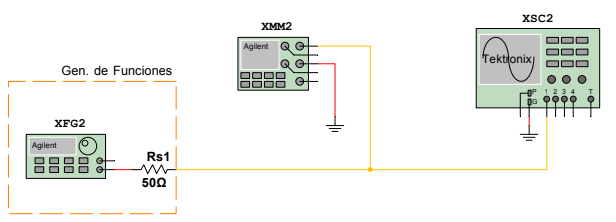
\includegraphics[width=0.8\textwidth]{diagramas/diagrama objetivo 1.PNG}
    \captionof{figure}{Diagrama del circuito para determinar amplitud y valor eficaz para distintas funciones.}
    \label{fig}
\end{Figura}

Se conectó el generador de funciones \textbf{Winstek SFG-2110} al osciloscopio \textbf{Agilent DS0362A} y el multímetro \textbf{Rigol DM3058}, después con la primer función (que fue senoidal) configurada y con un voltaje de salida de $1V$, con las opciones de measure en el osciloscopio se obtuvieron tanto el voltaje pico a pico $V_{pp}$ como el eficaz $V_{rms}$, con el multímetro también se obtuvo el valor eficaz, esto mismo se hizo para las otras funciones.

\subsection*{Objetivo 2}

\begin{Figura}
    \centering
    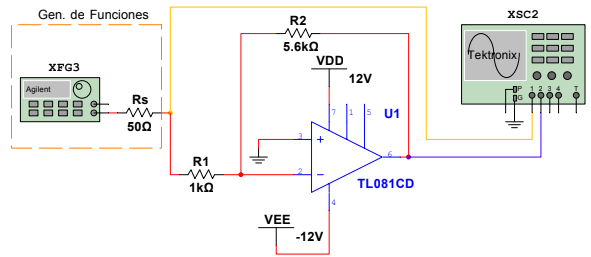
\includegraphics[width=0.8\textwidth]{diagramas/diagrama objetivo 2.PNG}
    \captionof{figure}{Diagrama del circuito para determinar el ancho de banda para el amplificador inversor.}
    \label{fig}
\end{Figura}

Se armó el circuito presente en el diagrama de la figura 2 sobre una protoboard, se utilizaron 2 resistencia de $1k\Omega$ y $5.6k \Omega$, una fuente bipolar de $\pm 12V$, un amplificador operacional \textbf{TL081CD} y cables. Con el circuito armado, se conectó el generador de funciones \textbf{Winstek SFG-2110} configurado con un voltaje de salida de $1V$ y una frecuencia de $100kHz$ y con una función senoidal se conectó la salida a la entrada del circuito, después se conecto el canal 1 del osciloscopio \textbf{Agilent DS0362A} en la salida del generador de funciones y el segundo canal en la salida del circuito armado. 

Con ayuda de las opciones de measure en el osciloscopio se midió el voltaje pico a pico $V_{pp}$ y se aumentó la frecuencia hasta tener un $V_{pp}$ igual al valor eficaz $V_{rms}$ que para una función senoidal es $\frac{V_{pp}}{\sqrt{2}}$ después se registro la frecuencia a la que se encontraba este voltaje. 

\subsection*{Objetivo 3}

\begin{Figura}
    \centering
    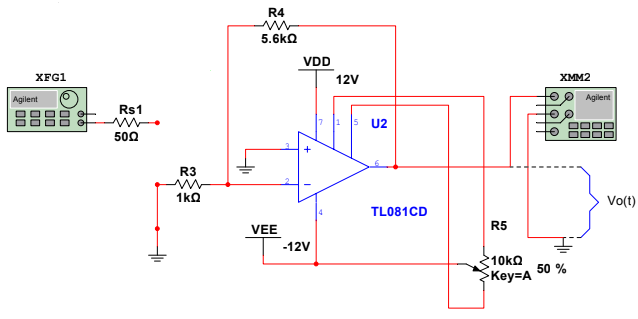
\includegraphics[width=0.8\textwidth]{diagramas/diagrama objetivo 2.1.PNG}
    \captionof{figure}{Diagrama del circuito anterior para balancearse.}
    \label{fig}
\end{Figura}

Para balancear el circuito se desconectó el generador de funciones y el osciloscopio del circuito de la figura 2 y se agregó un multímetro \textbf{Rigol DM3058} a la salida del operacional y un trimpot conectado así como se muestra en la figura 3, después con ayuda de un destornillador y con el multímetro ajustado para medir el voltaje de salida, se ajustó el trimpot de tal manera que el voltaje de salida mostrado en el multimetro fuera lo mas cercano al cero.

\subsection*{Objetivo 4}

\begin{Figura}
    \centering
    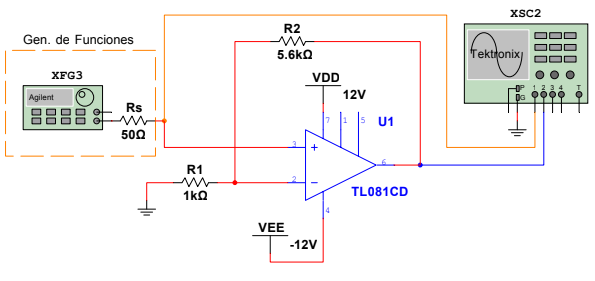
\includegraphics[width=0.8\textwidth]{diagramas/diagrama objetivo 3.PNG}
    \captionof{figure}{Diagrama del circuito para determinar el ancho de banda para el amplificador no inversor.}
    \label{fig}
\end{Figura}

Al igual que en el objetivo 2 se armó el circuito con los mismos materiales pero cambiando la entrada del operacional, se conectó el generador de funciones con la misma configuración que en el objetivo 2, también se usaron el canal 1 en la salida del generador de funciones y el 2 en la salida del operacional. Se midió el voltaje pico a pico $V_{pp}$ y se aumentó la frecuencia del generador de funciones hasta alcanzar aproximadamente el valor eficaz $V_{rms}$.

\subsection*{Objetivo 5}

\begin{Figura}
    \centering
    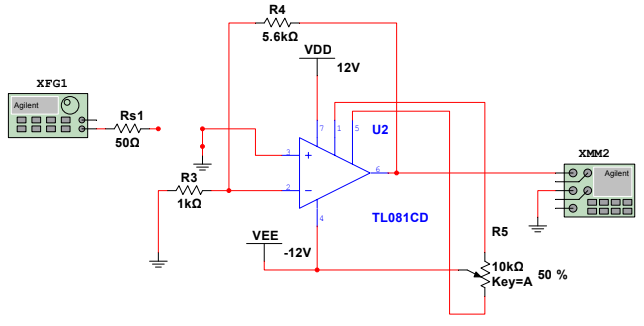
\includegraphics[width=0.8\textwidth]{diagramas/diagama objetivo 3.1.PNG}
    \captionof{figure}{Diagrama del circuito anterior para balancearse.}
    \label{fig}
\end{Figura}

Como en el objetivo 3, se balanceo el circuito desconectando el generador de funciones y conectando en la salida el multímetro, también se usó un trimpot y un destornillador para ajustar el mismo para que el voltaje de salida fuera lo mas cercano al cero.

\subsection*{Objetivo 6}

\begin{Figura}
    \centering
    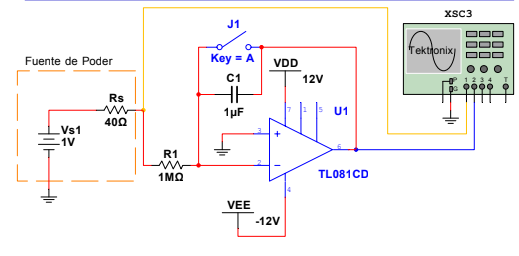
\includegraphics[width=0.8\textwidth]{diagramas/diagrama objetivo 4.PNG}
    \captionof{figure}{Diagrama del circuito para el amplificador inversor integrador.}
    \label{fig}
\end{Figura}

Se armó un circuito inversor integrador con un amplificador operacional \textbf{TL081} alimentado con una fuente bipolar de $\pm 12V$, un condensador de $1 \mu F$, una resistencia de $1 M \Omega$ y un interruptor. En la entrada del operacional se conectó una fuente de poder configurada con una salida de $1 V$ y $0.5 A$ y se conectó un osciloscopio tanto en la salida de la fuente de poder como en la salida del operacional para observar la función original y la integrada.

\subsection*{Objetivo 7}

\begin{Figura}
    \centering
    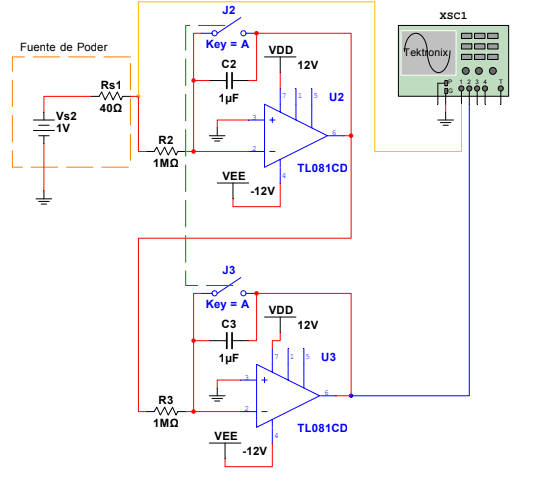
\includegraphics[width=0.8\textwidth]{diagramas/diagrama objetivo 5.PNG}
    \captionof{figure}{Diagrama del circuito para el doble inversor integrador.}
    \label{fig}
\end{Figura}

En el laboratorio presencial se intentó armar el doble integrador pero por diversos motivos el resultado no fue satisfactorio por lo que se decidió mejor hacer este objetivo en el simulador multisim, donde se siguieron los mismo pasos que en el objetivo anterior para hacer 2 inversores integradores conectados en cascada solo que usando un interruptor doble para cortocircuitar los 2 operacionales al mismo tiempo.



\section*{Resultados y Discusión}

\subsection*{Objetivo 1}

\begin{tabular}{|c|c|c|c|} 
 \hline
 Función  & $V_{m}$ & $V_{rms}$ \\ 
 \hline
 Senoidal  & 1.0305 V & 0.700626 V  \\  \hline
 Triangular  & 1.0205 V & 0.57716 V \\ \hline
 Cuadrada  & 1.1205 V & 1.098 V  \\ \hline
 Senoidal + c. de c.d & 1.0305 V & 1.672 V  \\ \hline

\end{tabular}

Para encontrar las incertidumbres de las correspondientes $V_{rms}$ utilicemos la tabla de incertidumbres para el multimetro, ubicada en el anexo:

\begin{equation*}
    \delta V_{rms1}=\pm(0.700626 \cdot 0.015\% + 200 \cdot (10)^{-3} \cdot 0.004\% ) V
\end{equation*}

\begin{equation*}
=\pm1.130939\times10^{-4}V
\end{equation*}

\begin{equation*}
    \delta V_{rms2}=\pm(0.57716 \cdot 0.015\% + 200 \cdot (10)^{-3} \cdot 0.004\% ) V
\end{equation*}

\begin{equation*}
=\pm0.94574\times10^{-4}V
\end{equation*}

\begin{equation*}
    \delta V_{rms3}=\pm(1.098 \cdot 0.015\% + 200 \cdot (10)^{-3} \cdot 0.004\% ) V
\end{equation*}

\begin{equation*}
=\pm1.727\times10^{-4}V
\end{equation*}

\begin{equation*}
    \delta V_{rms4}=\pm(1.672 \cdot 0.015\% + 200 \cdot (10)^{-3} \cdot 0.004\% ) V
\end{equation*}

\begin{equation*}
=\pm2.588\times10^{-4}V
\end{equation*}

Para encontrar las incertidumbres de las correspondientes $V_{m}$ utilicemos la tabla de incertidumbres para el osciloscopio, ubicada en el anexo:

\begin{equation*}
    \delta V_{m1}=\pm(3\% \cdot 1.0305 + 0.1 \cdot 500\times10^{-3}+1\times10^{-3} ) V
\end{equation*}

\begin{equation*}
    =\pm 0.081915 V
\end{equation*}

\begin{equation*}
    \delta V_{m2}=\pm(3\% \cdot 1.0205 + 0.1 \cdot 500\times10^{-3}+1\times10^{-3} ) V
\end{equation*}

\begin{equation*}
    =\pm 0.081615 V
\end{equation*}

\begin{equation*}
    \delta V_{m3}=\pm(3\% \cdot 1.1205 + 0.1 \cdot 500\times10^{-3}+1\times10^{-3} ) V
\end{equation*}

\begin{equation*}
    =\pm 0.084615 V
\end{equation*}

\begin{equation*}
    \delta V_{m4}=\pm(3\% \cdot 1.0305 + 0.1 \cdot 500\times10^{-3}+1\times10^{-3} ) V
\end{equation*}

\begin{equation*}
    =\pm 0.081915 V
\end{equation*}

\subsection*{Objetivo 2}

El voltaje de entrada fue:

\begin{equation*}
    v_{i} = 1.0805 V
\end{equation*}

Utilizando la tabla de incertidumbres para el osciloscopio encontramos que la incertidumbre de este valor es:

\begin{equation*}
    \delta v_{i}=\pm(3\%\cdot 1.0805 + 0.1 \cdot 500 (10)^{-3} + 1\times10^{-3} ) V
\end{equation*}

\begin{equation*}
    =\pm( 0.083415) V
\end{equation*}

La función utilizada tenia una frecuencia:

\begin{equation*}
    f= 1kHz
\end{equation*}

Esto nos dio un voltaje de salida:

\begin{equation*}
    v_{0} = 6.2 V
\end{equation*}

La incertidumbre de este valor es:

\begin{equation*}
    \delta v_{0}=\pm(3\%\cdot 6.2 + 0.1 \cdot 500 (10)^{-3} + 1\times10^{-3} ) V
\end{equation*}

\begin{equation*}
    =\pm( 0.237) V
\end{equation*}

Se aumentó la frecuencia hasta:

\begin{equation*}
    f= 353 kHz
\end{equation*}

Para esta frecuencia el voltaje de salida fue:

\begin{equation*}
    v'_{0} = 4.2505 V
\end{equation*}

La incertidumbre de este valor es:

\begin{equation*}
    \delta v'_{0}=\pm(3\%\cdot 4.2505 + 0.1 \cdot 500 (10)^{-3} + 1\times10^{-3} ) V
\end{equation*}

\begin{equation*}
    =\pm( 0.178515) V
\end{equation*}
$v'_{0}$ se mantuvo constante hasta la frecuencia:

\begin{equation*}
    f= 365 kHz
\end{equation*}

$v'_{0}$ corresponde a aproximadamente el $70.7\%$ del valor del voltaje pico $v_{0}$.
\\\\
Tomando el promedio de las frecuencias y tomando la incertidumbre como la distancia hasta sus extremos encontramos que al ancho de banda es:

\begin{equation*}
    f= \left(\frac{353+365}{2}\pm \left(\frac{353+365}{2}-353\right) \right) kHz
\end{equation*}

\begin{equation*}
    = (359\pm6) kHz
\end{equation*}

\subsection*{Objetivo 3}

La siguiente imagen muestra el circuito balanceado.

\begin{Figura}
    \centering
    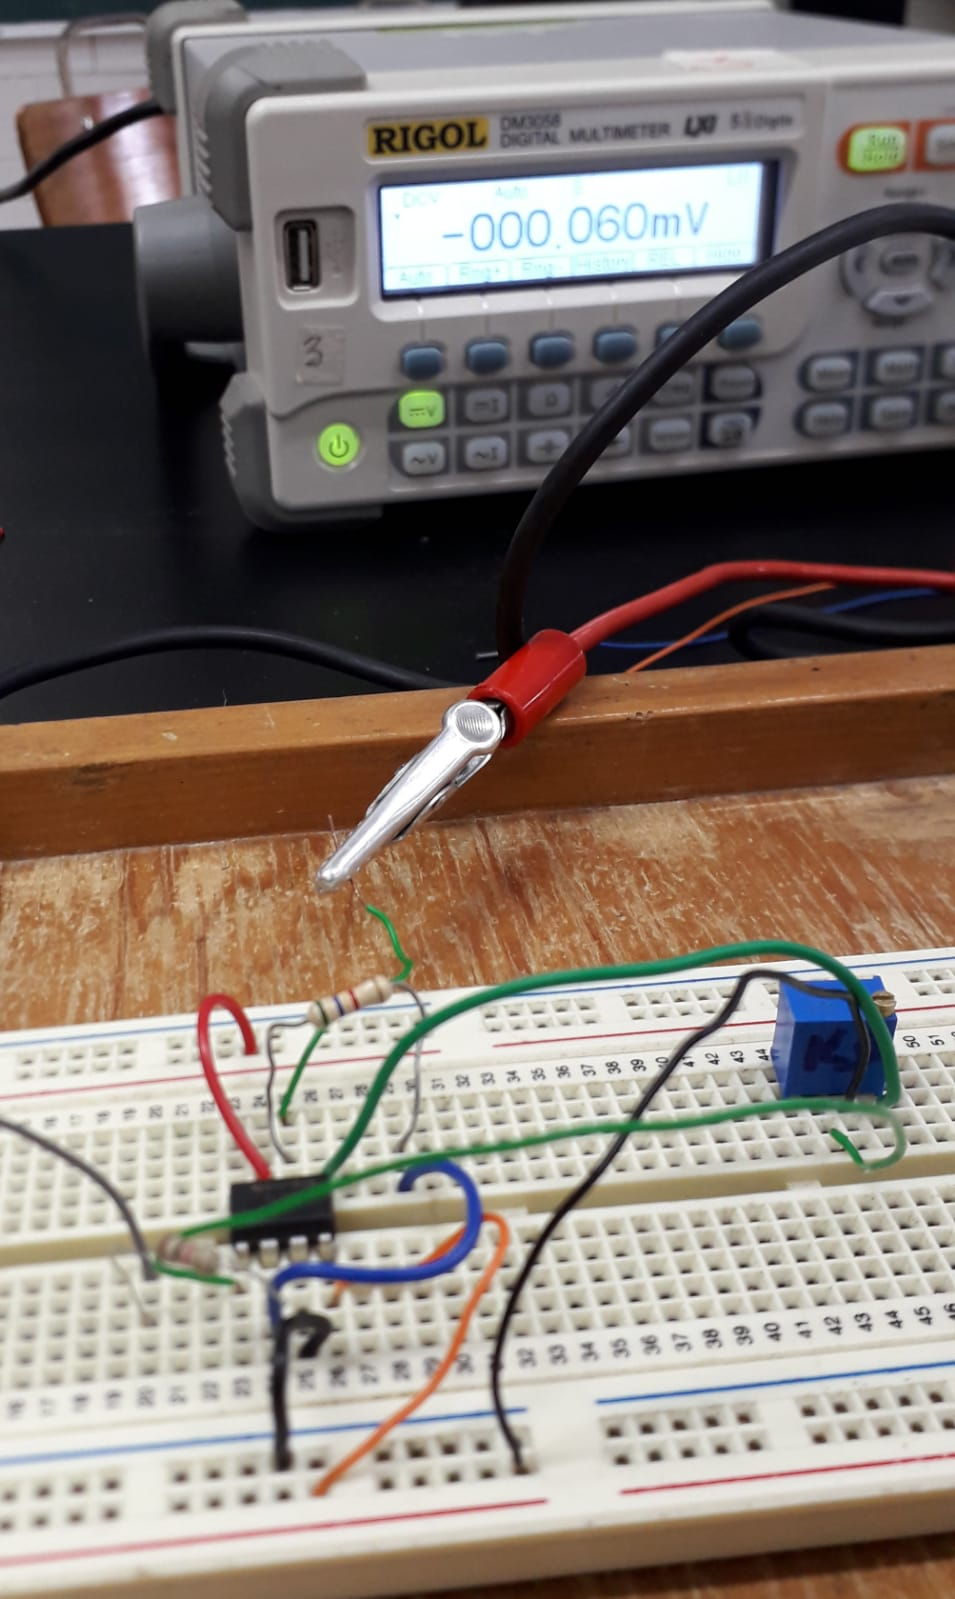
\includegraphics[width=0.7\textwidth]{Objetivo2Balancearimangen.jpeg}
    \captionof{figure}{}
    \label{fig}
\end{Figura}

\subsection*{Objetivo 4}

El voltaje de entrada fue:

\begin{equation*}
    v_{i} = 1.1205 V
\end{equation*}

Utilizando la tabla de incertidumbres para el osciloscopio encontramos que la incertidumbre de este valor es:

\begin{equation*}
    \delta v_{i}=\pm(3\%\cdot 1.1205 + 0.1 \cdot 500 (10)^{-3} + 1\times10^{-3} ) V
\end{equation*}

\begin{equation*}
    =\pm( 0.084615) V
\end{equation*}

La función utilizada tenia una frecuencia:

\begin{equation*}
    f= 1kHz
\end{equation*}

Esto nos dio un voltaje de salida:

\begin{equation*}
    v_{0} = 7.65 V
\end{equation*}

\begin{equation*}
    \delta v_{0}=\pm(3\%\cdot 7.65 + 0.1 \cdot 500 (10)^{-3} + 1\times10^{-3} ) V
\end{equation*}

\begin{equation*}
    =\pm( 0.2805) V
\end{equation*}

Se aumentó la frecuencia hasta:

\begin{equation*}
    f= 337 kHz
\end{equation*}

Para esta frecuencia el voltaje de salida fue:

\begin{equation*}
    v'_{0} = 5.2 V
\end{equation*}

\begin{equation*}
    \delta v'_{0}=\pm(3\%\cdot 5.2 + 0.1 \cdot 500 (10)^{-3} + 1\times10^{-3} ) V
\end{equation*}

\begin{equation*}
    =\pm( 0.207) V
\end{equation*}

$v'_{0}$ se mantuvo prácticamente constante hasta la frecuencia:

\begin{equation*}
    f= 343 kHz
\end{equation*}

$v'_{0}$ corresponde a aproximadamente al $70.7\%$ del valor del voltaje pico $v_{0}$.
\\\\
Tomando el promedio de las frecuencias y tomando la incertidumbre como la distancia hasta sus extremos encontramos que al ancho de banda es:
\begin{equation*}
    f= \left(\frac{337+343}{2}\pm \left(\frac{337+343}{2}-337\right) \right) kHz
\end{equation*}
\begin{equation*}
    = (340\pm3) kHz
\end{equation*}
\subsection*{Objetivo 5}

La siguiente imagen muestra el circuito anterior balanceado.

\begin{Figura}
    \centering
    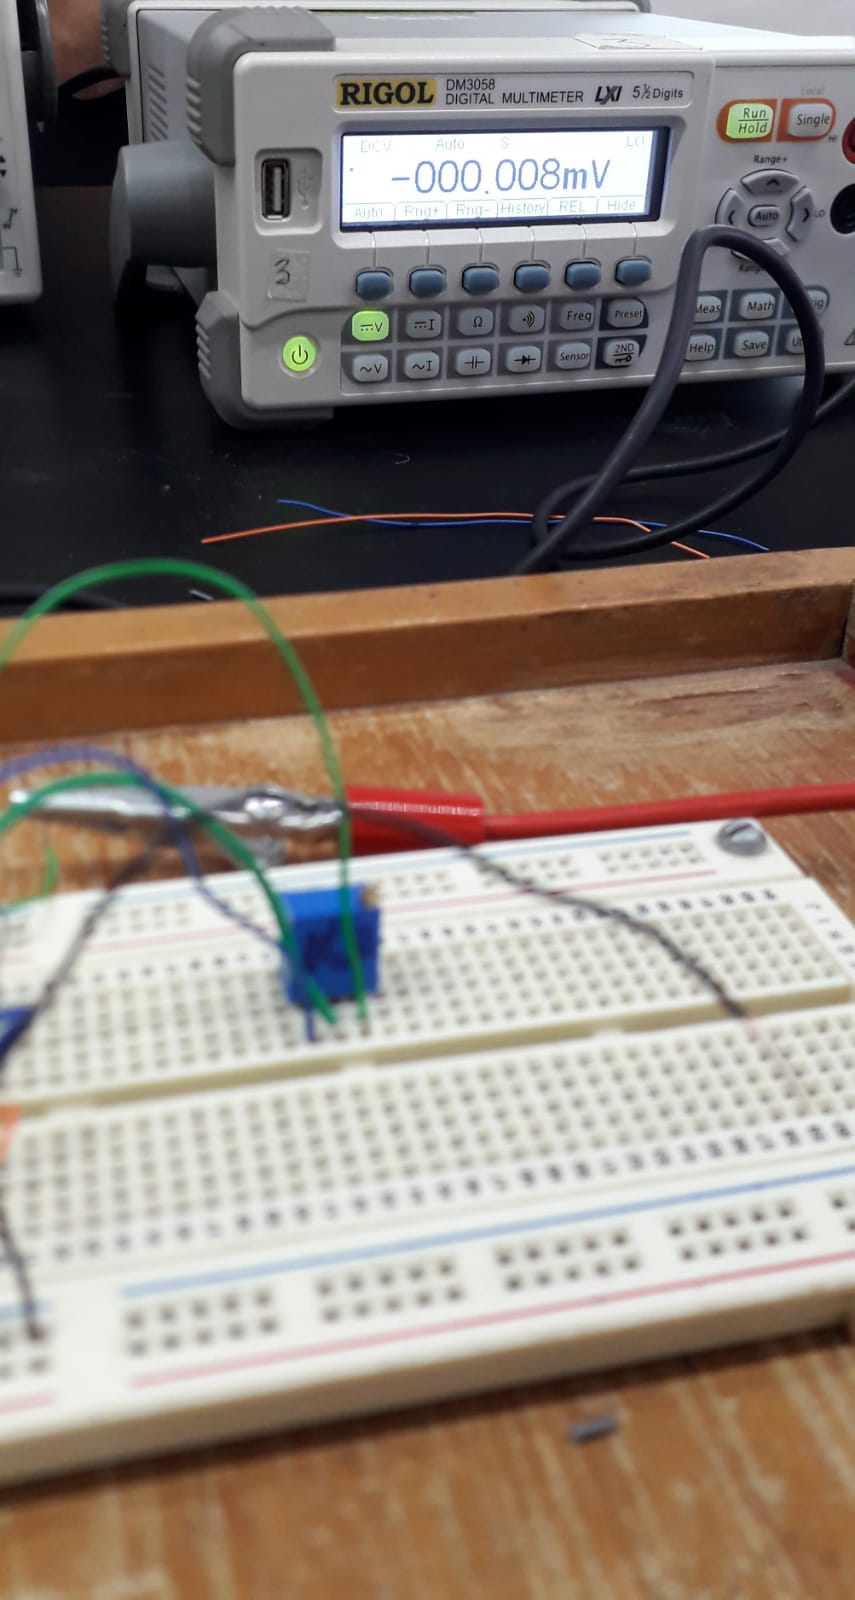
\includegraphics[width=0.7\textwidth]{Objetivo4Balancearimangen.jpeg}
    \captionof{figure}{Circuito balanceado.}
    \label{fig}
\end{Figura}

\subsection*{Objetivo 6}

Se construyo el amplificador inversor integrador, el osciloscopio mostró lo siguiente:

\begin{Figura}
    \centering
    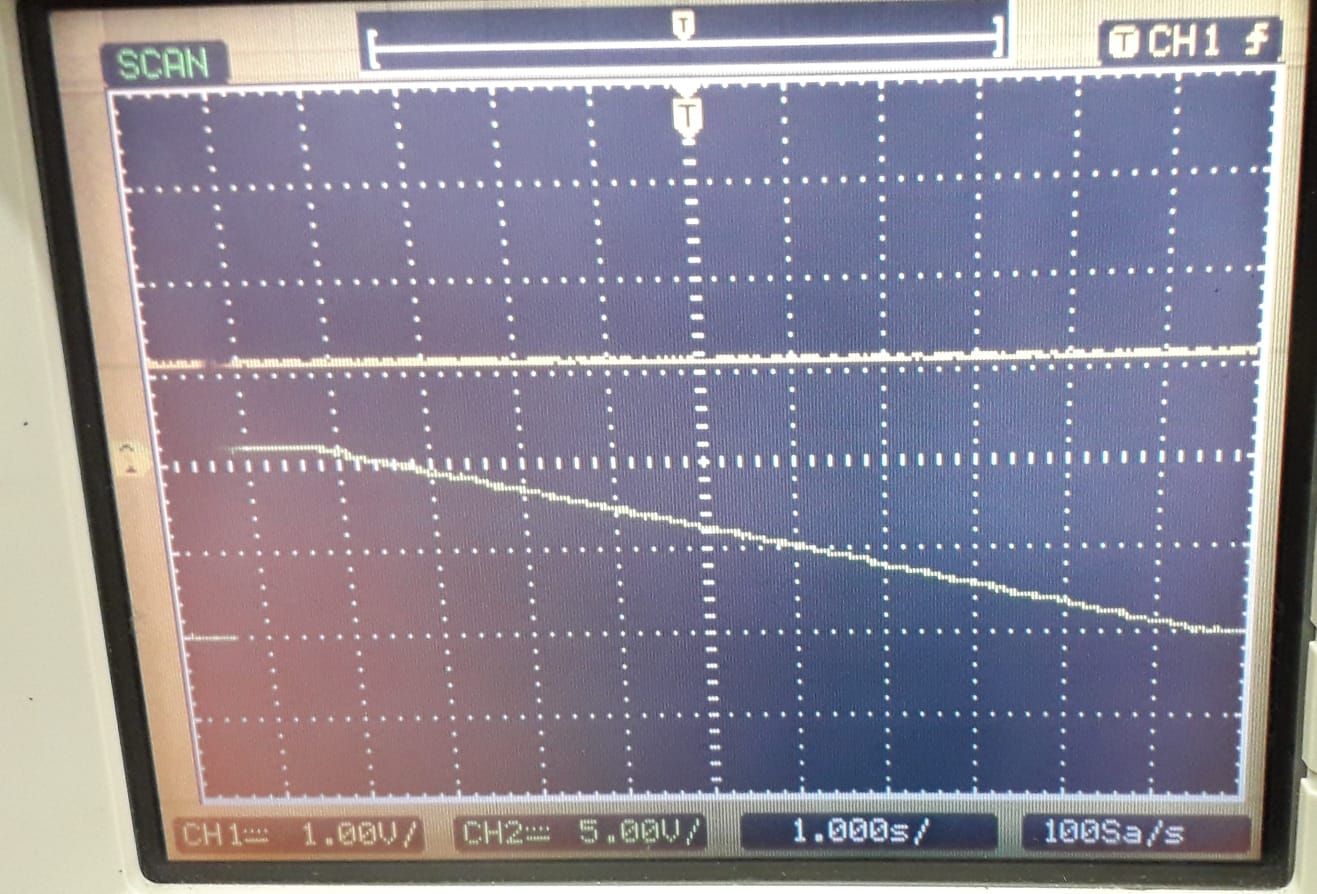
\includegraphics[width=0.8\textwidth]{OsciloscipioIntegrador.jpeg}
    \captionof{figure}{Gráfica del integrador.}
    \label{fig}
\end{Figura}

\subsection*{Objetivo 7}

Se construyo el doble integrador en multisim por falta de tiempo, el osciloscopio mostró lo siguiente:

\begin{Figura}
    \centering
    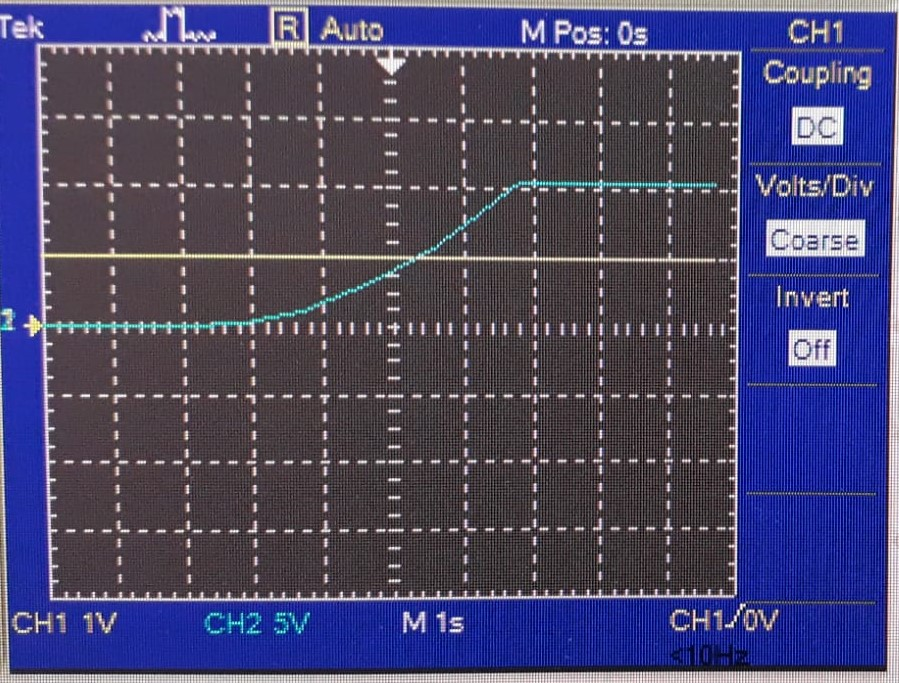
\includegraphics[width=0.8\textwidth]{OsciloscipioDobleIntegrador.jpeg}
    \captionof{figure}{Grafica doble integrador}
    \label{fig}
\end{Figura}

\section*{Conclusiones}
\subsection*{Objetivo 1}
Se obtuvo la amplitud $V_{m}$ y el valor eficaz $V_{rms}$ para diferentes funciones, los valores se muestran en la tabla $1$.

\subsection*{Objetivo 2}
  El ancho de banda para el amplificador inversor es:
  
  \begin{equation*}
    f= (359\pm6) kHz
\end{equation*}

\subsection*{Objetivo 3}
El circuito se balanceo correctamente.

\subsection*{Objetivo 4}

  El ancho de banda para el amplificador no inversor es:
  
  \begin{equation*}
    f= (340\pm3) kHz
\end{equation*}

\subsection*{Objetivo 5}
El circuito se balanceo correctamente.

\subsection*{Objetivo 6}
Se construyo correctamente el amplificador inversor integrador.

\subsection*{Objetivo 7}
Se construyo correctamente el doble integrador en multisim.

\begin{thebibliography}{99}
\bibitem{2} William Hart Hayt, Jack Ellsworth Kemmerly, Jamie D Phillips, and Steven M Durbin. 2019. Análisis de Circuitos En Ingeniería. Ciudad De México Mcgraw Hill Interamericana S.A. De C.V.

\bibitem{2} Floyd, Thomas L. Principios De Circuitos eléctricos (8a. Ed.). Naucalpan de Juárez: Pearson Educación, 2007.
\end{thebibliography}

\section*{Apéndices}

\end{multicols}

\begin{Figura}
    \centering
    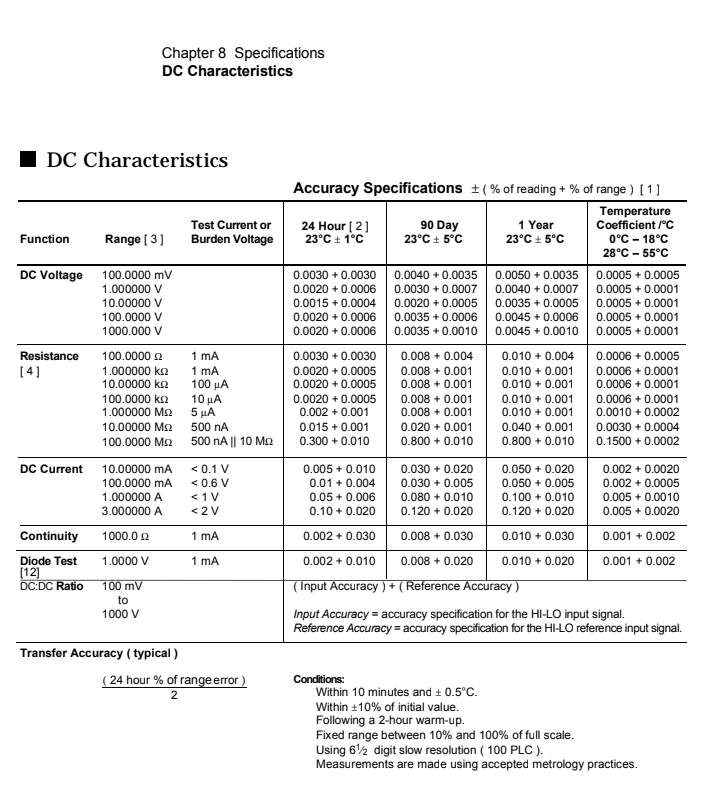
\includegraphics[width=1\textwidth]{incertidumbres multimetro.PNG}
    \captionof{figure}{Tabla de incertidumbres para el multímetro Rigol DM3058}
    \label{fig}
\end{Figura}

\begin{Figura}
    \centering
    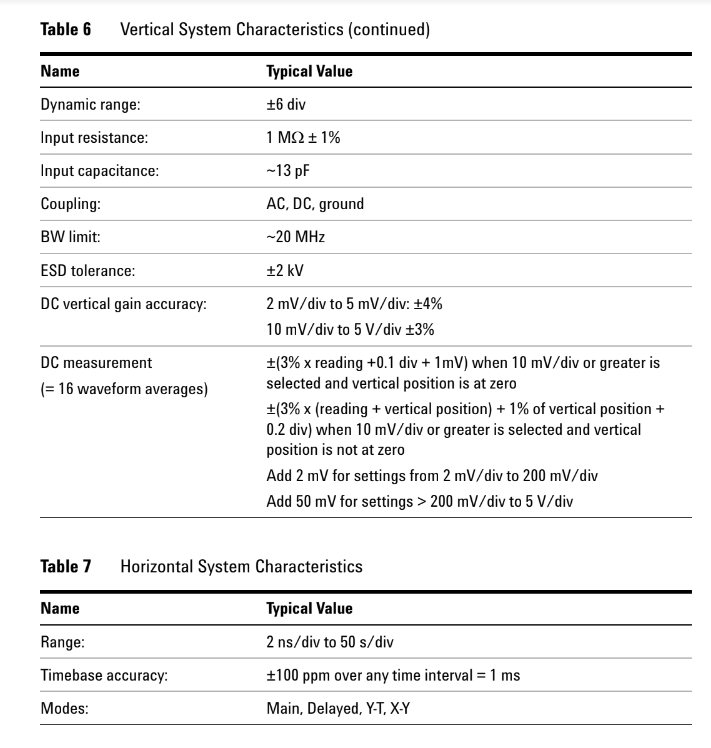
\includegraphics[width=1\textwidth]{incertidumbres osciloscopio.png}
    \captionof{figure}{Tabla de incertidumbres para el osciloscopio Agilent DS0362A}
    \label{fig}
\end{Figura}

\end{document}